\documentclass[aspectratio=169]{beamer}

% Minimal packages
\usepackage{graphicx}
\usepackage{hyperref}
\usepackage{amsmath}
\usepackage{fontspec}
\setsansfont{Helvetica} 

\usepackage{tikz}
\usepackage{tikz-cd}
\usetikzlibrary{mindmap}
\usepackage{quiver}


% Minimal design; compile with XeLaTeX or LuaLaTeX.
\definecolor{slideBlue}{HTML}{03057C}
\definecolor{slideInk}{HTML}{202124}
\definecolor{slideMuted}{HTML}{777777}
\usetheme{default}
\setbeamersize{text margin left=1cm,text margin right=1cm}
\setbeamercolor{background canvas}{bg=white}
\setbeamercolor{normal text}{fg=slideInk,bg=white}
\setbeamercolor{structure}{fg=slideBlue}
\setbeamercolor{block body}{fg=slideInk,bg=white}
\setbeamercolor{block title}{fg=slideBlue,bg=white}
\setbeamercolor{title}{fg=white}
\setbeamercolor{subtitle}{fg=white}
\setbeamerfont{title}{size=\fontsize{26}{30}\selectfont,series=\bfseries}
\setbeamerfont{subtitle}{size=\fontsize{12}{16}\selectfont,series=\mdseries}
\setbeamertemplate{navigation symbols}{}
\setbeamertemplate{headline}{}
\setbeamertemplate{frametitle}{}
\setbeamertemplate{itemize item}{\small\textbullet}
\setbeamertemplate{itemize subitem}{\scriptsize\textbullet}
\setbeamertemplate{footline}{%
    \hfill{\color{slideMuted}\scriptsize\insertframenumber}%
    \hspace*{1cm}\vspace*{0.35cm}
}
\setbeamertemplate{section in toc}[sections numbered]
\setbeamertemplate{subsection in toc}[subsections numbered]
\setbeamercolor{section in toc}{fg=slideInk}
\setbeamercolor{subsection in toc}{fg=slideMuted}
\AtBeginEnvironment{frame}{\raggedright}

\newcommand{\slideheading}[1]{%
    {\small\bfseries\color{slideMuted}#1\par}
    \vspace{1em}
}

% Place \sectiondivider after a \section command only where a divider is wanted.
\newcommand{\sectiondivider}{%
    \begingroup
    \setbeamercolor{background canvas}{bg=slideBlue}
    \begin{frame}[plain,noframenumbering]
        \vfill
        {\color{white}\huge\bfseries\MakeUppercase{\insertsectionhead}\par}
        \vfill
    \end{frame}
    \endgroup
}

% Title
\title{\uppercase{Toward Categorical\\Information Science}}
\subtitle{Boundary Objects, Comparative Epistemolology, and Sheafification }
% \subtitle{A Compositional and Critical Framework for  Knowledge Representation, Conceptual Modeling, and Cybernetic/System Thinking}

\author{Ngozi Harrison \\ ngozih@g.ucla.edu}
\date{Dec 2026 \\  \small {}}
\institute{Field Notes : Stack Exchange}

% Image macro (kept but simple)
\newcommand{\myimage}[1]{%
    \begin{center}%
        \includegraphics[width=0.6\textwidth, clip=true]{assets/#1}\par
    \end{center}%
}

% Hyperref settings
\hypersetup{
    pdfauthor={Ngozi Harrison},
    pdftitle={},
    colorlinks=false,
    linkcolor=blue,
    urlcolor=blue
}

\begin{document}

% Title Slide

    \begingroup
    \setbeamercolor{background canvas}{bg=slideBlue}
    \setbeamertemplate{background}{%
        \begin{tikzpicture}[remember picture,overlay]
            \clip (current page.south west) rectangle (current page.north east);
            \node[anchor=center,inner sep=0pt,opacity=0.2]
                at (current page.center) {%
                    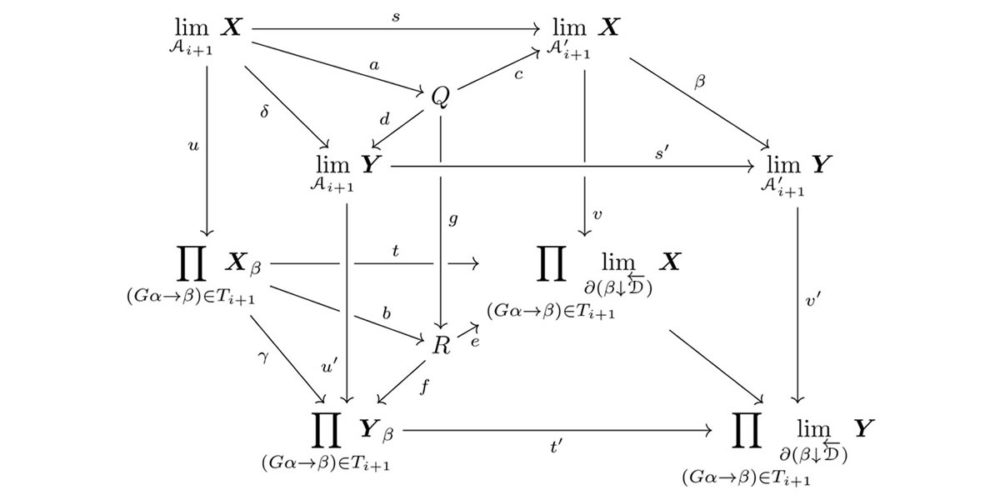
\includegraphics[height=\paperheight]{bgimage}%
                };
        \end{tikzpicture}%
    }
    \begin{frame}[plain,noframenumbering]
        \vspace*{0.8cm}
        {\usebeamerfont{title}\usebeamercolor[fg]{title}\inserttitle\par}
        \vspace{0.6cm}
        \begin{minipage}{0.88\textwidth}
            \raggedright
            \usebeamerfont{subtitle}\usebeamercolor[fg]{subtitle}
            \insertsubtitle\par
        \end{minipage}
        \vfill
        {\color{white}\small
            \insertauthor\par
            \vspace{0.4cm}
            \insertinstitute\par
            \insertdate\par
        }
        \vspace*{0.3cm}
    \end{frame}
    \endgroup


\begin{frame}
\slideheading{Overview}
\tableofcontents
\end{frame}

\begin{frame}
    \centering
    \vfill

    \setbeamercolor{quote box}{fg=slideInk,bg=white}
    \makebox[\textwidth][c]{%
        \begin{beamercolorbox}[wd=0.88\textwidth,sep=1.2em,center,rounded=false]{quote box}
            {\color{slideBlue}\fontsize{36}{36}\selectfont\bfseries ``\par}
            \vspace{-0.4em}

            {\large\itshape
            To us power is, first of all, the ability to define phenomena, and secondly the ability to make these phenomena act in a desired manner.\par}

            \vspace{1em}
            {\small\mdseries\centering
            --- Huey Newton\par}
        \end{beamercolorbox}%
    }

    \vfill
\end{frame}

\begin{frame}
    \begin{columns}[c,onlytextwidth]
        \column{0.55\textwidth}
        \centering
        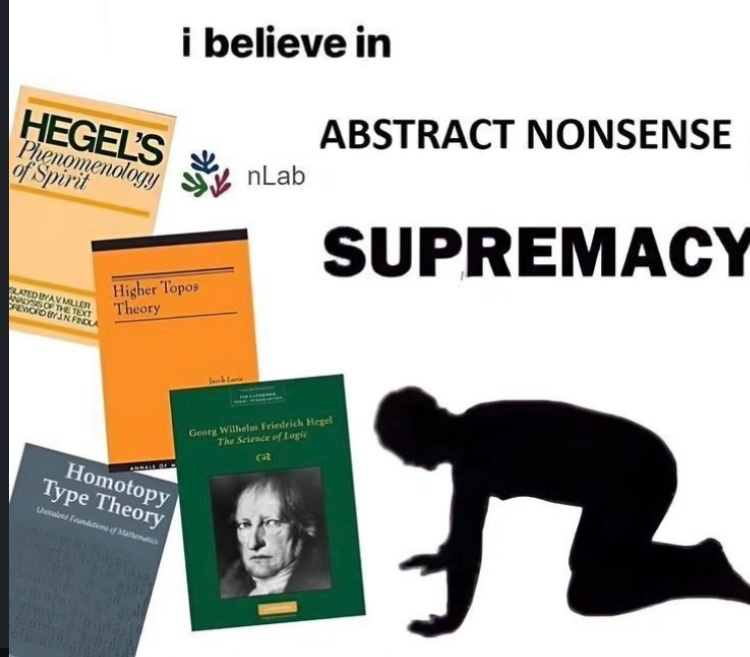
\includegraphics[width=\linewidth,height=0.72\textheight,keepaspectratio]{IMG_0440}
        \column{0.40\textwidth}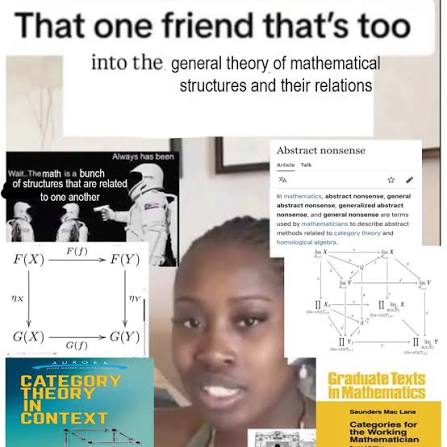
\includegraphics[width=\linewidth,height=0.92\textheight,keepaspectratio]{images(14)}
    \end{columns}
\end{frame}



\begin{frame}
    \centering
    \vfill

    \setbeamercolor{quote box}{fg=slideInk,bg=white}
    \makebox[\textwidth][c]{%
        \begin{beamercolorbox}[wd=0.88\textwidth,sep=1.2em,center,rounded=false]{quote box}
            {\color{slideBlue}\fontsize{36}{36}\selectfont\bfseries ``\par}
            \vspace{-0.4em}

            {\large\itshape
            The language of categories is affectionately known as ``abstract nonsense,''
            so named by Norman Steenrod. This term is essentially accurate and not
            necessarily derogatory: categories refer to ``nonsense'' in the sense that
            they are all about the ``structure,'' and not about the ``meaning,'' of what
            they represent.\par}

            \vspace{1em}
            {\small\mdseries\centering
            --- Paolo Aluffi, \textit{Algebra: Chapter 0}\par}
        \end{beamercolorbox}%
    }

    \vfill
\end{frame}



\section{Motivation}
\sectiondivider
\begin{frame}
	\slideheading{Motivation}
	Categorical Information Science is my attempt to think at the intersection of philosophy, information science, and applied category theory at three abstract levels
	\begin{itemize}
		\item level of concept
		\item level of problem
		\item level of system
	\end{itemize}
	In this presentation I present an assemblage of ideas, examples and provocations for thinking about ways that Applied category theory can inform theorizing, modeling, and scientific practice. 
\end{frame}


\begin{frame}
	The Aristotilian and Set theoretic Legacy of Information Science
	While we don't often focus explicitly on mathematics and logic within information science, there is a hidden legacy which informs much of thinking and practice within IS
\end{frame}

\begin{frame}
	\slideheading{Our Aristotilian Legacy}
	
\end{frame}

\section{Philosophical Preliminaries}
\sectiondivider

\begin{frame}
	The reading list
	\begin{itemize}
		\item Sylvia Wynter
		\item Yuk Hui
		\item Hegel
		\item Robert Brandom
		\item Celia Lury
		\item Lawvere \& Schanuel
		\item Eugenia Cheng
		\item Alain Badiou
		\item Emily Reihl
		\item David Spivak
		\item Brendan Fong
		\item ...
	\end{itemize}
\end{frame}

\begin{frame}
	\slideheading{What is a boundary object?}
	“Boundary objects are those objects that are plastic enough to be adaptable across multiple viewpoints, yet maintain continuity of identity.” \\ 
(The Structure of Ill-Structured Solutions: Boundary Objects and Heterogeneous Distributed Problem Solving, p. 243)
\end{frame}

\begin{frame}
    \centering
    \vfill
    {\color{slideBlue}\small\bfseries  TAKEAWAY}\par
    \vspace{1em}
    {\color{slideInk}\LARGE\bfseries
   Boundary objects are fundamentally compositional, \\ \large{thus thinking in a generative way about boundary objects requires a framework for thinking with compositionality}}
    \vfill
\end{frame}

\section{The Categorical Paradigm}
\sectiondivider

\begin{frame}
    \centering
    \vfill

    \setbeamercolor{quote box}{fg=slideInk,bg=white}
    \makebox[\textwidth][c]{%
        \begin{beamercolorbox}[wd=0.88\textwidth,sep=1.2em,center,rounded=false]{quote box}
            {\color{slideBlue}\fontsize{36}{36}\selectfont\bfseries ``\par}
            \vspace{-0.4em}

            {\large\itshape
           Mathematical objects are determined by--and understood by--the network of relationships they enjoy with all the other objects of their species.\par}

            \vspace{1em}
            {\small\mdseries\centering
            --- Barry Mazur \par}
        \end{beamercolorbox}%
    }

    \vfill
\end{frame}



\section{What is Category Theory?}
\sectiondivider


\begin{frame}
    \slideheading{Category theory: a map of the basic concepts}
    \centering
    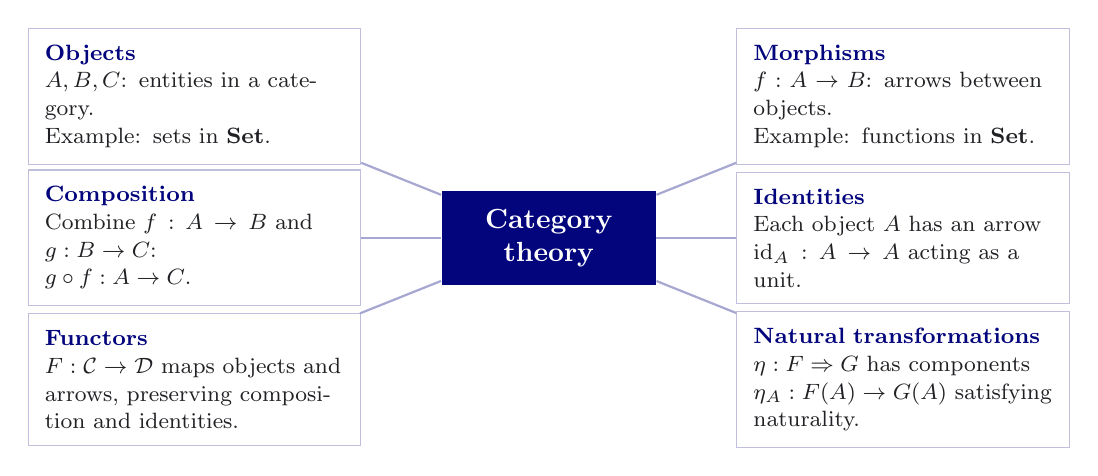
\begin{tikzpicture}[
        topic/.style={
            draw=slideBlue!25,
            sharp corners,
            fill=white,
            text=slideInk,
            text width=3.8cm,
            minimum height=1.3cm,
            inner sep=6pt,
            align=left,
            font=\fontsize{8}{10}\selectfont
        },
        connection/.style={draw=slideBlue!35,line width=0.8pt}
    ]
        \node[
            fill=slideBlue,text=white,sharp corners,
            text width=2.3cm,minimum height=1.2cm,
            align=center,font=\normalsize\bfseries,inner sep=6pt
        ] (category) at (0,0) {Category theory};

        \node[topic] (objects) at (-4.5,1.8) {
            \textbf{\color{slideBlue}Objects}\par
            $A,B,C$: entities in a category.\par
            Example: sets in $\mathbf{Set}$.
        };
        \node[topic] (morphisms) at (4.5,1.8) {
            \textbf{\color{slideBlue}Morphisms}\par
            $f:A\to B$: arrows between objects.\par
            Example: functions in $\mathbf{Set}$.
        };
        \node[topic] (composition) at (-4.5,0) {
            \textbf{\color{slideBlue}Composition}\par
            Combine $f:A\to B$ and $g:B\to C$:\par
            $g\circ f:A\to C$.
        };
        \node[topic] (identities) at (4.5,0) {
            \textbf{\color{slideBlue}Identities}\par
            Each object $A$ has an arrow\par
            $\mathrm{id}_A:A\to A$ acting as a unit.
        };
        \node[topic] (functors) at (-4.5,-1.8) {
            \textbf{\color{slideBlue}Functors}\par
            $F:\mathcal{C}\to\mathcal{D}$ maps objects and arrows,
            preserving composition and identities.
        };
        \node[topic] (natural) at (4.5,-1.8) {
            \textbf{\color{slideBlue}Natural transformations}\par
            $\eta:F\Rightarrow G$ has components\par
            $\eta_A:F(A)\to G(A)$ satisfying naturality.
        };
        \draw[connection] (category) -- (objects);
        \draw[connection] (category) -- (morphisms);
        \draw[connection] (category) -- (composition);
        \draw[connection] (category) -- (identities);
        \draw[connection] (category) -- (functors);
        \draw[connection] (category) -- (natural);
    \end{tikzpicture}
    \par\vspace{0.4em}
    {\footnotesize
        \textbf{\color{slideBlue}Category laws}\quad
        $h\circ(g\circ f)=(h\circ g)\circ f$
        \qquad
        $\mathrm{id}_B\circ f=f=f\circ\mathrm{id}_A$
        \par
        \vspace{0.3em}
        Objects and arrows live within categories; functors connect categories;
        natural transformations connect parallel functors.
    }
\end{frame}


\begin{frame}
	\slideheading{Common mathematical domains and the categorical viewpoint}
	\centering
    \begingroup
    \renewcommand{\arraystretch}{1.5}
    \setlength{\tabcolsep}{6pt}
    \small
    \begin{tabular}{@{}p{0.20\textwidth}p{0.33\textwidth}p{0.37\textwidth}@{}}
        \hline
        \textbf{\color{slideBlue}Category} &
        \textbf{\color{slideBlue}Objects} &
        \textbf{\color{slideBlue}Morphisms} \\
        \hline
        Set &
        sets  &
        functions \\
        Group &
        groups  &
        group homomorphisms \\
        Coproduct $A+B$ &
        Injections from $A$ and $B$ &
        Disjoint union with source tags \\
        \hline
    \end{tabular}
    \par
    \endgroup
\end{frame}


\section{Applied Category Theory}
\sectiondivider
% Sheaves, Topoi, and Modeling Behavior

\begin{frame}
	Themes
	\begin{itemize}
		\item category theory as a model of models
		\item functorial semantics
		\item compositionality
	\end{itemize}
\end{frame}

\section{Knowledge Representation using Ologs}
\sectiondivider


\section{Sheafification and Comparative Epistemology}
\sectiondivider

\begin{frame}
\slideheading{Presheaves and Sheaves}	
\begin{columns}[T,onlytextwidth]
        \column{0.48\textwidth}
        \begin{beamercolorbox}[wd=\linewidth,sep=0pt]{block body}
            {\large\bfseries\color{slideBlue}Concept space}\par
            \vspace{0.5em}
            What are the entities and distinctions in the domain?
            \begin{itemize}
                \item concepts
                \item relations
                \item categories
            \end{itemize}
        \end{beamercolorbox}
        \column{0.48\textwidth}
        \begin{beamercolorbox}[wd=\linewidth,sep=0pt]{block body}
            {\large\bfseries\color{slideBlue}Problem space}\par
            \vspace{0.5em}
            What question or difficulty are we trying to address?
            \begin{itemize}
                \item goals
                \item constraints
                \item evidence
            \end{itemize}
        \end{beamercolorbox}
    \end{columns}
\end{frame}


\begin{frame}
	\slideheading{Sheafification}
	Sheafification is a process of transforming a presheaf into a sheaf by forcing local information to satisfy global rules and gluing conditions
	
	
\end{frame}
\begin{frame}
	Zalamea adapts sheafification from a mathematical method to tool for thinking about ontology and epistemology. He argues that the development of the concept of the sheaf marks a key break between modern mathematics and contemporary mathematics and uses this concept to elaborate a perspective and philosophical methodology for thinking comparatively and sythentically.
\end{frame}

\section{Sheaffification and Comparative Epistemology}

\section{Categorical cybernetics}
\sectiondivider

\section{Socialism???}
\sectiondivider


\begin{frame}
    \slideheading{Logic of Worlds}
    \begin{columns}[c,onlytextwidth]
        \column{0.55\textwidth}
        \centering
        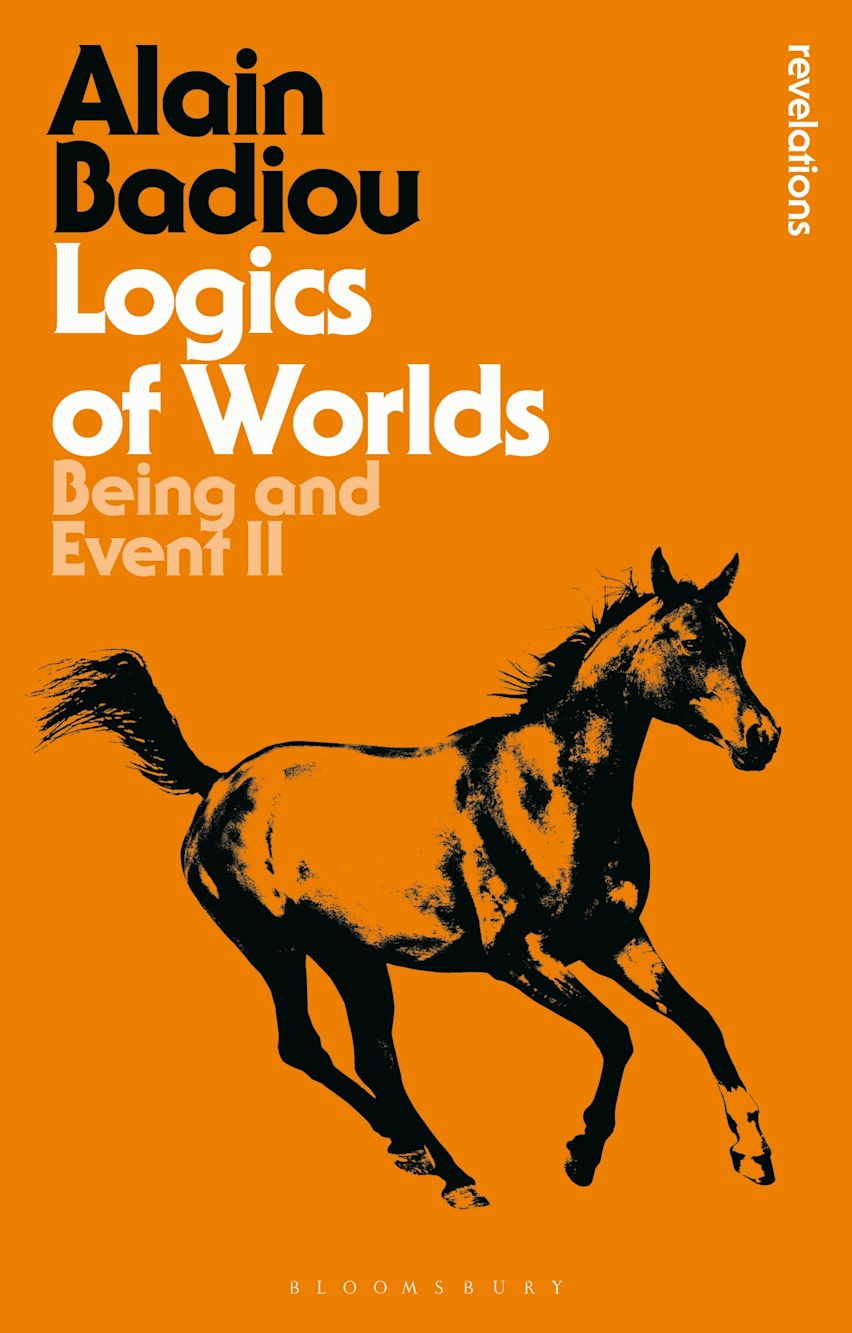
\includegraphics[width=\linewidth,height=0.62\textheight,keepaspectratio]{logicofworlds.jpg}\par
        \vspace{0.8em}
         {\small\color{slideMuted}“The human animal is the being \\ of the thousand logics” \\ (Badiou, 2009, pg 69).\par}
        \column{0.40\textwidth}
        {\Large\bfseries\color{slideInk}Logic of Worlds by Alain Badiou}\par
        \vspace{0.8em}
        In his second entry in the being and event series Badiou complements his set theoretic ontology of pure being with a systematic philosophy of appearance, phenomenology and worlds using category theory. 
       
    \end{columns}
\end{frame}

\begin{frame}
    \slideheading{Logic and Appearance}
    There is no single universal logic that governs appearance, instead there are many worlds governed by logics
    \vspace{0.4em}
    \begin{columns}[T,onlytextwidth]
        \column{0.48\textwidth}
        \begin{beamercolorbox}[wd=\linewidth,sep=0pt]{block body}
            {\large\bfseries\color{slideBlue}Logic}\par
            \vspace{0.5em}
            What are the entities and distinctions in the domain?
            \begin{itemize}
                \item concepts
                \item relations
                \item categories
            \end{itemize}
        \end{beamercolorbox}
        \column{0.48\textwidth}
        \begin{beamercolorbox}[wd=\linewidth,sep=0pt]{block body}
            {\large\bfseries\color{slideBlue}Appearance}\par
            \vspace{0.5em}
            Worlds are formalized as categories where objects appear according to a transcendental, an algebra that assigns degrees of exisstence to objects and their relations. 
            \begin{itemize}
                \item goals
                \item constraints
                \item evidence
            \end{itemize}
        \end{beamercolorbox}
    \end{columns}
\end{frame}

\begin{frame}
	\slideheading{Objective Phenomenology and the Logic of Capital}
	Phenomenology typically focuses on how things appear to the consciousness of a human subject.\par
	\vspace{0.8em}
	\textbf{Objective Phenomenology} Suspends the subject and focuses on how objects and social forms appear to each other in the logic of a specific world.
\end{frame}

\begin{frame}
	\slideheading{Marx as Objective Phenomenologist}
	 Marx critique of commodity fetishism points us to how systemic relations between things are reduced human perceptions of seeminly innate properties\par
	 \vspace{0.8em}
	 Gabriel Tupinamba, Yuan Yao 
\end{frame}

\appendix

\section{Appendix}
\sectiondivider

\begin{frame}
    \slideheading{Two-column comparison}
    \begin{columns}[T,onlytextwidth]
        \column{0.48\textwidth}
        \begin{beamercolorbox}[wd=\linewidth,sep=0pt]{block body}
            {\large\bfseries\color{slideBlue}Concept space}\par
            \vspace{0.5em}
            What are the entities and distinctions in the domain?
            \begin{itemize}
                \item concepts
                \item relations
                \item categories
            \end{itemize}
        \end{beamercolorbox}
        \column{0.48\textwidth}
        \begin{beamercolorbox}[wd=\linewidth,sep=0pt]{block body}
            {\large\bfseries\color{slideBlue}Problem space}\par
            \vspace{0.5em}
            What question or difficulty are we trying to address?
            \begin{itemize}
                \item goals
                \item constraints
                \item evidence
            \end{itemize}
        \end{beamercolorbox}
    \end{columns}
\end{frame}

\begin{frame}
    \slideheading{Three-step process}
    \centering
    \begin{columns}[c,onlytextwidth]
        \column{0.30\textwidth}
        \begin{beamercolorbox}[wd=\linewidth,sep=0pt,center]{block body}
            {\Large\bfseries\color{slideBlue}01}\par
            \vspace{0.5em}
            \textbf{Observe}\par
            Identify the domain and its questions.
        \end{beamercolorbox}
        \column{0.30\textwidth}
        \begin{beamercolorbox}[wd=\linewidth,sep=0pt,center]{block body}
            {\Large\bfseries\color{slideBlue}02}\par
            \vspace{0.5em}
            \textbf{Model}\par
            Represent concepts and relationships.
        \end{beamercolorbox}
        \column{0.30\textwidth}
        \begin{beamercolorbox}[wd=\linewidth,sep=0pt,center]{block body}
            {\Large\bfseries\color{slideBlue}03}\par
            \vspace{0.5em}
            \textbf{Reflect}\par
            Test what the model makes visible.
        \end{beamercolorbox}
    \end{columns}
\end{frame}

\begin{frame}
    \slideheading{Image with a takeaway}
    \begin{columns}[c,onlytextwidth]
        \column{0.55\textwidth}
        \centering
        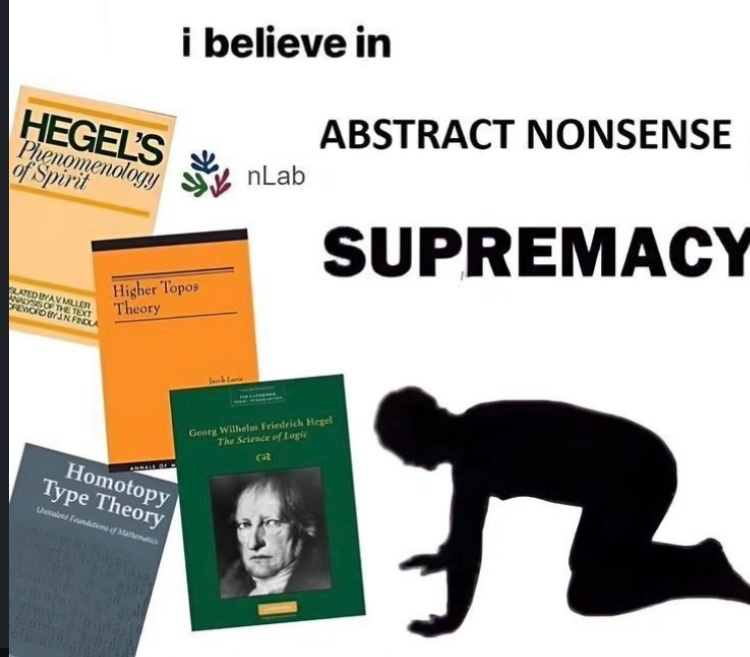
\includegraphics[width=\linewidth,height=0.62\textheight,keepaspectratio]{IMG_0440}
        \column{0.40\textwidth}
        {\Large\bfseries\color{slideInk}A visual can do more than decorate.}\par
        \vspace{0.8em}
        Use the image to establish a setting, then connect it to one clear claim.
        \vspace{0.8em}

        {\small\color{slideMuted}Image caption or source goes here.}
    \end{columns}
\end{frame}

\begin{frame}
    \slideheading{Evidence and interpretation}
    \begin{columns}[T,onlytextwidth]
        \column{0.45\textwidth}
        {\large\bfseries\color{slideBlue}Observation}\par
        \vspace{0.5em}
        A model groups several distinct cases under the same category.
        \begin{itemize}
            \item What is included?
            \item What is left out?
        \end{itemize}
        \column{0.06\textwidth}
        \centering
        {\Large\color{slideBlue}$\rightarrow$}
        \column{0.45\textwidth}
        {\large\bfseries\color{slideBlue}Interpretation}\par
        \vspace{0.5em}
        Classification choices shape what can be compared, counted, or acted upon.
        \begin{itemize}
            \item State the implication.
            \item Name the limitation.
        \end{itemize}
    \end{columns}
\end{frame}

\begin{frame}
    \centering
    \vfill
    {\color{slideBlue}\small\bfseries ONE TAKEAWAY}\par
    \vspace{1em}
    {\color{slideInk}\LARGE\bfseries
    Models do not only describe a world.\\
    They help determine what we can ask of it.}
    \vfill
\end{frame}

\begin{frame}
    \slideheading{Math: definition and interpretation}
    \begin{columns}[T,onlytextwidth]
        \column{0.52\textwidth}
        {\large\bfseries\color{slideBlue}Functor}\par
        A functor $F:\mathcal{C}\to\mathcal{D}$ maps objects and
        morphisms while preserving identities and composition:
        \[
            F(\mathrm{id}_X)=\mathrm{id}_{F(X)}
        \]
        \[
            \boxed{F(g\circ f)=F(g)\circ F(f)}
        \]
        \column{0.43\textwidth}
        {\large\bfseries\color{slideBlue}What this means}\par
        \begin{itemize}
            \item Objects become objects.
            \item Arrows become arrows.
            \item Composing before or after translation gives the same result.
        \end{itemize}
    \end{columns}
\end{frame}

\begin{frame}
    \slideheading{Math: a step-by-step derivation}
    Let $F:\mathcal{C}\to\mathcal{D}$ and
    $G:\mathcal{D}\to\mathcal{E}$ be functors, with composable
    arrows $f:X\to Y$ and $g:Y\to Z$.
    \begin{align*}
        (G\circ F)(g\circ f)
            &=G\bigl(F(g\circ f)\bigr) \\
            &=G\bigl(F(g)\circ F(f)\bigr) \\
            &=G(F(g))\circ G(F(f)) \\
            &=(G\circ F)(g)\circ(G\circ F)(f).
    \end{align*}
    {\color{slideBlue}\bfseries Takeaway:}
    the composite preserves composition. Identity preservation follows
    similarly, so $G\circ F$ is a functor.
\end{frame}

\begin{frame}
    \slideheading{Table: comparing categorical constructions}
    \centering
    \begingroup
    \renewcommand{\arraystretch}{1.5}
    \setlength{\tabcolsep}{6pt}
    \small
    \begin{tabular}{@{}p{0.20\textwidth}p{0.33\textwidth}p{0.37\textwidth}@{}}
        \hline
        \textbf{\color{slideBlue}Construction} &
        \textbf{\color{slideBlue}Data} &
        \textbf{\color{slideBlue}Interpretation in sets} \\
        \hline
        Product $A\times B$ &
        Projections to $A$ and $B$ &
        All pairs $(a,b)$ \\
        Pullback $A\times_C B$ &
        Maps $f:A\to C$, $g:B\to C$ &
        Pairs with $f(a)=g(b)$ \\
        Coproduct $A+B$ &
        Injections from $A$ and $B$ &
        Disjoint union with source tags \\
        \hline
    \end{tabular}
    \par
    \endgroup
    \vspace{1em}
    {\small These constructions are characterized by universal properties,
    not just by their set-theoretic realizations.}
\end{frame}

\begin{frame}
    \slideheading{Diagram: a commutative square}
    \begin{columns}[c,onlytextwidth]
        \column{0.48\textwidth}
        \[
        \begin{tikzcd}[ampersand replacement=\&,row sep=large,column sep=large]
            A \arrow[r,"f"] \arrow[d,"h"'] \&
            B \arrow[d,"k"] \\
            C \arrow[r,"g"'] \& D
        \end{tikzcd}
        \]
        \column{0.47\textwidth}
        {\large\bfseries\color{slideBlue}Two paths to the same place}\par
        Starting at $A$ and ending at $D$, either path gives the same morphism:
        \[
            \boxed{k\circ f=g\circ h}
        \]
        Commutativity is a condition on the arrows, not just a feature of
        how they are drawn.
    \end{columns}
\end{frame}

\begin{frame}
    \slideheading{Diagram: the universal property of a product}
    \begin{columns}[c,onlytextwidth]
        \column{0.53\textwidth}
        \[
        \begin{tikzcd}[ampersand replacement=\&,column sep=1.3em,row sep=large]
            \& X
                \arrow[dl,"u"']
                \arrow[d,dashed,"{\exists!\,\langle u,v\rangle}" description]
                \arrow[dr,"v"] \& \\
            A \& A\times B \arrow[l,"\pi_A"] \arrow[r,"\pi_B"'] \& B
        \end{tikzcd}
        \]
        \column{0.42\textwidth}
        For every pair $u:X\to A$ and $v:X\to B$, there is a
        \textbf{unique} mediating arrow such that
        \[
            \begin{aligned}
                \pi_A\circ\langle u,v\rangle&=u,\\
                \pi_B\circ\langle u,v\rangle&=v.
            \end{aligned}
        \]
        {\small In sets: $\langle u,v\rangle(x)=(u(x),v(x))$.}
    \end{columns}
\end{frame}

\begin{frame}
    \slideheading{Diagram: naturality as compatibility}
    Let $F,G:\mathcal{C}\to\mathcal{D}$ be functors.
    A natural transformation $\eta:F\Rightarrow G$ assigns an arrow
    $\eta_X:F(X)\to G(X)$ to each object $X$.
    \[
    \begin{tikzcd}[ampersand replacement=\&,row sep=large,column sep=huge]
        F(X) \arrow[r,"F(f)"] \arrow[d,"\eta_X"'] \&
        F(Y) \arrow[d,"\eta_Y"] \\
        G(X) \arrow[r,"G(f)"'] \& G(Y)
    \end{tikzcd}
    \]
    For every $f:X\to Y$, the square commutes:
    \[
        G(f)\circ\eta_X=\eta_Y\circ F(f).
    \]
\end{frame}

\begin{frame}
% https://q.uiver.app/#q=WzAsNCxbMCwwLCJQIl0sWzIsMCwiWSJdLFswLDIsIlgiXSxbMiwyLCJaIl0sWzAsMSwicF8xIl0sWzIsMywiZiJdLFswLDIsInBfMiIsMV0sWzEsMywiZyIsMV1d
\[\begin{tikzcd}[ampersand replacement=\&]
	P \&\& Y \\
	\\
	X \&\& Z
	\arrow["{p_1}", from=1-1, to=1-3]
	\arrow["{p_2}"{description}, from=1-1, to=3-1]
	\arrow["g"{description}, from=1-3, to=3-3]
	\arrow["f", from=3-1, to=3-3]
\end{tikzcd}\]

\end{frame}




\end{document}
